\documentclass[12pt]{article}
\usepackage{amsmath}
\usepackage{graphicx}
\usepackage{hyperref}
\usepackage[utf8]{inputenc}
\usepackage{geometry}
\usepackage{mathtools}
\usepackage{empheq}
\usepackage{listings}
\usepackage{xcolor}
\usepackage{caption}
\usepackage{subcaption}
\usepackage{setspace}
\usepackage{indentfirst}
\usepackage{authblk}
\usepackage{svg}

\graphicspath{ {./assets/} }
\geometry{margin=1in}
\doublespacing
\captionsetup{labelfont=bf}

\title{CHEN 425 Workshop 1}
\author{Mark Levchenko}
\date{25 January 2023}

\begin{document}

% Info %%%%%%%%%%%%%%%%%%%%%%%%%%%%%%%%%%%%%%%%%%%%%%%%%%%%

\textbf{CHEN 425 ASPEN Simulation Report}

\textbf{Title:} Sensitivity Analysis

\textbf{Workshop:} \#5

\textbf{Date:} 8 March, 2023

\textbf{Prepared by:} Mark Levchenko

\textbf{To:} Professor Mahmoud El-Halwagi


% Report %%%%%%%%%%%%%%%%%%%%%%%%%%%%%%%%%%%%%%%%%%%%%%%%%%%%
\section{Summary of Results}
\subsection{Part A}

The dew point of the flash separator is 274 $^\circ$F, the same result as Workshop \#2.

\subsection{Part B}

The maximumm allowable pressure for the compressor is 120 psia, the same as Workshop \#1.

\subsection{Part C}

To improve on the operating costs of the distillation column from Workshop \#3, the reflux ratio and pressure could be adjusted so that less heating and cooling is required. Decreasing the reflux ratio and pressure resulted in lower heating and cooling usage, decreasing the operating cost of the column.

\section{Discussion of Simulation Results}

\subsection{Part A}

\begin{center}
    \includesvg[scale=0.8]{assets/parta_plot.svg}
\end{center}

The dew point temperature occurs when the vapor fraction changes to 1. From the plot, the dew point is approximately 274 $^\circ$F. This result is identical to the one found in Workshop \#2.

\subsection{Part B}

\begin{center}
    \includesvg[scale=0.8]{assets/partb1_plot.svg}
\end{center}

From the plot above, the pressure at 640 $^\circ$F for the compressor is 120 psi. If the temperature of the compressor cannot exceed 640 $^\circ$F, then the maximum allowable pressure is 120 psi. This result is identical to the one found in Workshop \#3.

\begin{center}
    \includesvg[scale=0.8]{assets/partb2_plot.svg}
\end{center}

The above plot shows the brake power of the compressor as a function of pressure. Because the compressor is isentropic, the power required to drive it should change linearly with pressure. The plot verifies this realtionship as it is a straight line. 

\subsection{Part C}

The plots below show the total column duty as a function of various manipulated variables. The total column duty is the sum of the heating and cooling duties. This metric represents the total energy needed to drive the column. A higher total column duty results in higher operating costs and vice versa.

\begin{center}
    \includesvg[scale=0.8]{assets/partc1_plot.svg}
\end{center}

\begin{center}
    \includesvg[scale=0.8]{assets/partc2_plot.svg}
\end{center}

The total column duty increases as the mass reflux ration increases because the amount of liquid that needs to be vaporized increases. Also, the column duty increaes as the pressure increaes because the energy needed to vaporize a lquid increases as pressure increases. Therefore, in order to decrease the operating cost of the column, the pressure and reflux ratio should be decreased if possible.

\section{Simulation Screenshots}

\subsection{Part A}

Main flowsheet:

\begin{center}
    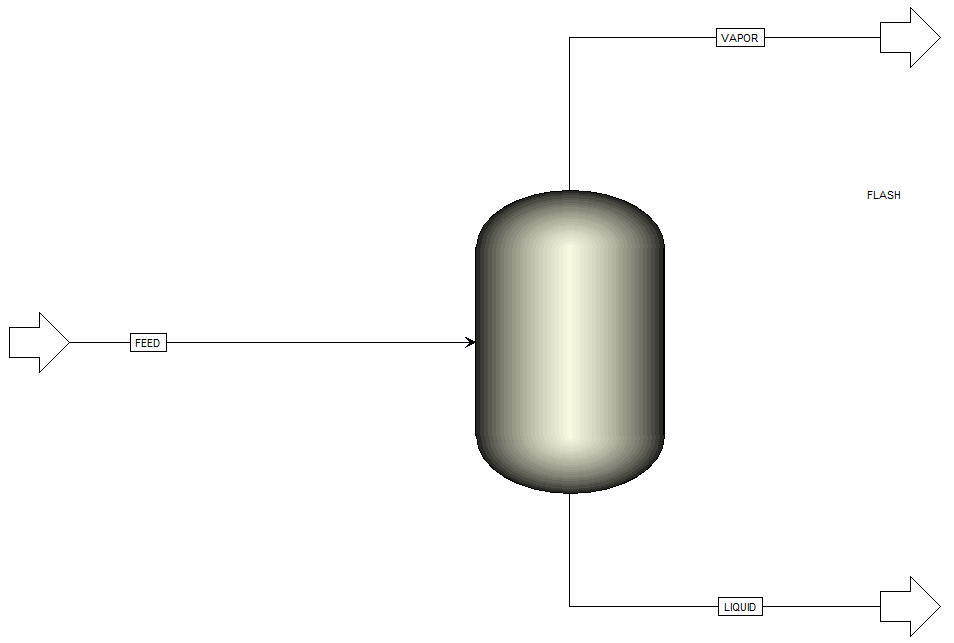
\includegraphics[width=0.9\textwidth]{assets/flow2.png}
\end{center}

\subsection{Part B}

Main flowsheet:

\begin{center}
    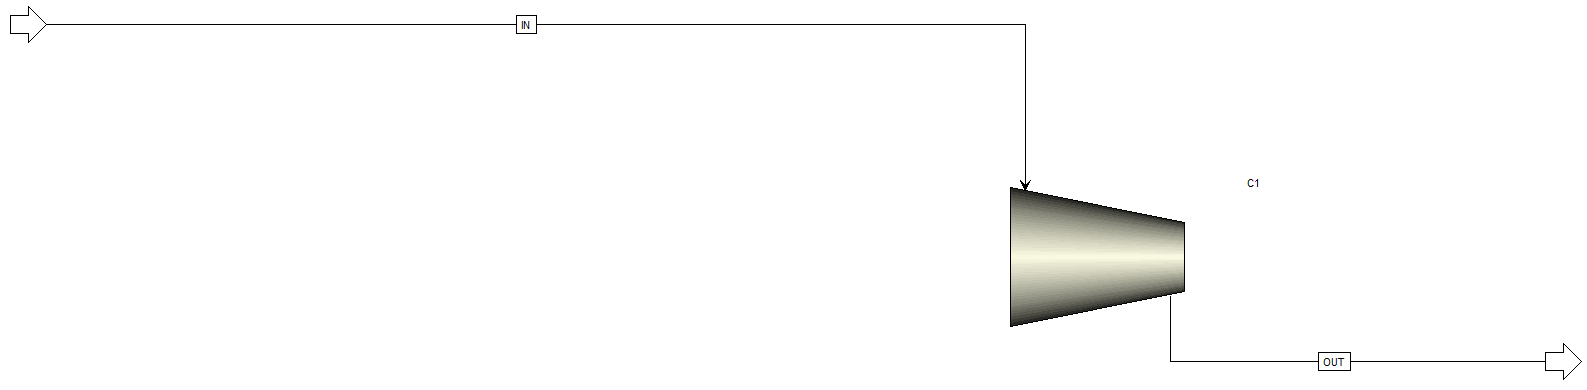
\includegraphics[width=0.9\textwidth]{assets/flow1.png}
\end{center}

\subsection{Part C}

Main flowsheet:

\begin{center}
    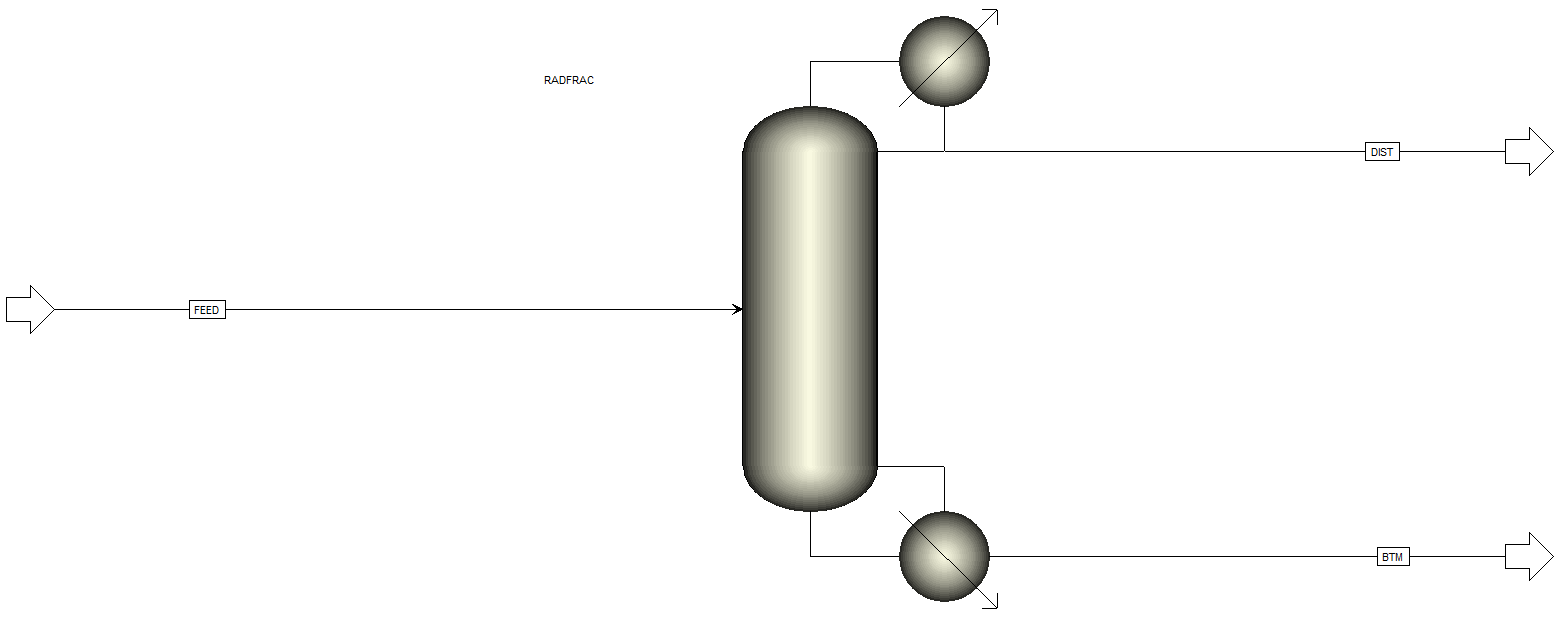
\includegraphics[width=0.9\textwidth]{assets/flow3.png}
\end{center}

\section{Conclusions}

Performing a sensitivity is a method for finding certain properties of a process or discovering optimizations. For example, in Workshop \#1, the maximum discharge pressure of a compressor needed to be found. Using a sensitivity analysis to plot the temperature as a function of the discharge pressure of the compressor allowed the maximum temperature to be obtained. Similarly, in Workshop \#2, the dew point in a flash separator was obtained. To find the dew point, a sensitivity analysis was performed plotting the temperature of the separator against the vapor fraction.

Optimization is another use for sensitivity analysis. Recomendations for a distillation column were created by performing a sensitivity analysis of its energy usage. The mass reflux ratio and pressure of the distillation column were plotted against the total energy usage of the column. From the plots, it was determined that decreasing the operating pressure and the mass reflux ratio of the column would decrease its energy usage, and thus decrease its operating cost.

\end{document}